% Copyright (C) 2018 by latexstudio <http://www.latexstudio.net>
%
% This program is free software: you can redistribute it and/or modify
% it under the terms of the GNU General Public License as published by
% the Free Software Foundation, either version 3 of the License, or
% (at your option) any later version.
%
% This program is distributed in the hope that it will be useful,
% but WITHOUT ANY WARRANTY; without even the implied warranty of
% MERCHANTABILITY or FITNESS FOR A PARTICULAR PURPOSE.  See the
% GNU General Public License for more details.
%
% You should have received a copy of the GNU General Public License
% along with this program.  If not, see <http://www.gnu.org/licenses/>.
%

\section{介绍公式的常见问题}


\faq{\cs{[} \ldots \cs{]} 与 \texttt{\$\$\ldots \$\$} 有什么区别?}{}

重定义的难度不同、造成的间距也不同。推荐使用 \cs{[} \ldots \cs{]}。 

参见
\url{https://www.zhihu.com/question/27589739/answer/37255728}


\faq{如何让长公式自动断行?}{}

长公式自动断行要看情况,如果是在行内模式,合理使用空格,一般可以在二元运算符处断行,如果是行间模式,推荐使用align类环境,在需要断行处添加|\\|%
%\textbackslash{} 
手动断行。


\faq{公式希腊字符如何加粗?}{}

希腊字母没有粗体,可以选择合适的数学字体。 可以使用 bm
宏包将希腊字母加粗。


\faq{极限符号下面有两个趋近该怎么写}{}

直接给出例子:

%\begin{verbatim}
\begin{example}
\[ \lim_{n\to\infty\atop m\to\infty} \]
\end{example}
%\end{verbatim}
%效果如下:
%
%\[ \lim_{n\to\infty\atop m\to\infty} \]
%\begin{Example}
%	\[ \lim_{n\to\infty\atop m\to\infty} \]
%\end{Example}

%\begin{example}
%	$\frac{1}{\pi}$,\quad
%	$\sqrt[5]{1+k^2+k^4}$
%\end{example}

%\begin{Example}
%	$\frac{1}{\pi}$,\quad
%	$\sqrt[5]{1+k^2+k^4}$
%\end{Example}

或者使用 \cs{substack},代码如下:

%\begin{verbatim}
%\documentclass{article}
%\usepackage{amsmath}
%\begin{document}
%\[ \lim_{\substack{n\to\infty\\ m\to\infty}} \]
%\end{document}
%\end{verbatim}
%
%效果如下:
%
%\[ \lim_{\substack{n\to\infty\\ m\to\infty}} \]
\begin{example}
\[ \lim_{\substack{n\to\infty\\ m\to\infty}} \]
\end{example}
 
% \includegraphics{https://images-cdn.shimo.im/FCY4A1SeBIcwBCGT/双重极限.PNG!thumbnail}


\faq{怎样在 LaTeX 中输入引号}{}

左引号用 `(键盘1旁边那个键),右引号用 `。双引号也一样,``''。
中文条件下可以直接用中文引号(这个与编码方式和中文支持方式有关的),会有自动配对(这个和编辑器以及输入法有关的),但是如果需要用到不配对引号的情况,需要使用通用方法。


\faq{align环境默认是居中对齐吗?我在使用时,发现公式开始是居中的,后来却一直靠右断对齐,这是什么原因?}{}

%\sout{align 默认靠右对齐,所以通常加 \&
%符号,让代码左对齐。验证一下以下代码:}

%\begin{verbatim}
%\begin{align}
%& \nabla \times H = J,\\
%& \nabla \times E = - \partial _t B,\\
%& \nabla \cdot B = 0.
%\end{align}
%\end{verbatim}
\begin{example}
\begin{align}
& \nabla \times H = J,\\
& \nabla \times E = - \partial _t B,\\
& \nabla \cdot B = 0.
\end{align}
\end{example}

再试试把 \& 去掉什么样。

align采用的是奇偶对齐的方式,第一列右对齐,第二列左对齐,就这样右左右左依此类推,两列之间用\&分隔。


\faq{中英文标点使用规则不是很明白,尤其在公式环境里,字体和间距差别都比较大。怎样才能让正文和公式的标点统一(形状和间隔)?}{}

详见:
\url{https://link.zhihu.com/?target=http\%3A//www.moe.gov.cn/ewebeditor/uploadfile/2015/01/13/20150113092346124.pdf}

在导言区加类似命令可实现全文替换:

\begin{verbatim}
\catcode`\。=\active\newcommand{。}{. }
\end{verbatim}

或者使用 xeCJK 宏包的字符映射功能,调用 fullwidth-stop
这一映射文件,将中文空心句号映射为实心句点:

\begin{verbatim}
\documentclass{article}
\usepackage{xeCJK}
\setCJKmainfont[Mapping= fullwidth-stop]{STSong}
\begin{document}
句号。
\end{document}
\end{verbatim}


\faq{公式如何居左对齐,居右对齐?}{}

公式居左对齐在基础文档类中由 fleqn
选项控制,选择该选项后,正文公式均居左对齐,至于居右对齐,嗯,我没见过这么奇怪的格式。


\faq{公式之后解释公式符号的文字,通常是 ``符号 ------ 解释'' 这样的格式,我希望这段文字的格式是按破折号对齐,并且解释文字折行后悬挂缩进,怎样实现这样的格式?}{}

方法很多,可以列表,可以align等环境。 这里给出一个使用自定义列表的例子:

\begin{verbatim}
\usepackage{ifthen}
\newcounter{qlst}
\newenvironment{EqDesc}[2][式中]{%
\begin{list}{}
 {%
  \usecounter{qlst}
  \settowidth{\labelwidth}{#1,\ \ #2\ --- \ }
  \setlength{\labelsep}{0pt}
  \setlength{\leftmargin}{\labelwidth}
  \setlength{\rightmargin}{0em}
  \setlength{\parsep}{0ex}
  \setlength{\itemsep}{0ex}
  \setlength{\itemindent}{0em}
  \setlength{\listparindent}{0em}
  \renewcommand{\makelabel}[1]
    {\stepcounter{qlst}
     \ifthenelse{\value{qlst}>1}{\hfill ##1\ --- \ }{#1,\hfill ##1\ --- \ }
    }
 }%
}%
{\end{list}}
\end{verbatim}

EqDesc
环境有两个参数,第一个为可选参数,是解释公式符号前的引导词,默认是``式中'',第二个参数是样本符号,可以选择一个列表中宽度最大的符号。条目 \cs{item} 有一个可选参数(实际使用是必选参数),内容是要说明的符号。使用如下:

%\begin{verbatim}
\begin{example}
\[ a^2+b^2=c^2 \]
\begin{EqDesc}[其中]{$a$}
   \item[$a$] 三角形的一条直角边;
   \item[$b$] 三角形的另一条直角边;
   \item[$c$] 三角形的斜边。
\end{EqDesc}
\end{example}
%\end{verbatim}

%{\centerline{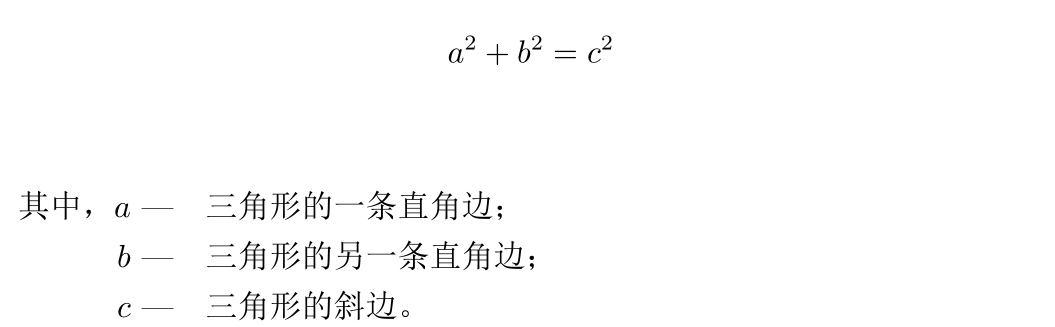
\includegraphics[width=0.8\linewidth]{include/images/hang}}}


\faq{行内公式的情况下如何让sum prod这些运算符的上下标在头上和脚下?}{}

这样处理行内公式的上下标会导致段落行距不整齐,不符合 \LaTeX{}
的审美。如果彻底放弃审美,可以使用 \cs{limits} 命令,如:

%\begin{verbatim}
\begin{example}
$\sum\limits_{i=1}^n, \prod\limits_\epsilon$
\end{example}
%\end{verbatim}

%效果是这样的:$\sum\limits_{i=1}^n \quad \prod\limits_\epsilon$

\faq{如何将积分的上限标放在积分号的上下两侧?}{}

积分号的上下限放置在积分号的右侧是英美国家和 \LaTeX{}
的排版习惯,通常无需处理。
如果你很确定需要按照 ISO 80000-2:2009 或者 GB 3102.11-93 的规定排版积分号,可以:

\begin{enumerate}
\def\labelenumi{\arabic{enumi}.}

\item
  在调用 amsmath 宏包时添加 intlimits 选项;
\item
  \texttt{\cs{def}\cs{int}\{\cs{intop}\}}
\item
  如果使用 unicode-math 宏包,
\end{enumerate}

%\begin{latexcode}
\begin{verbatim}
\removenolimits{%
  \int\iint\iiint\iiiint\oint\oiint\oiiint
  \intclockwise\varointclockwise\ointctrclockwise\sumint
  \intbar\intBar\fint\cirfnint\awint\rppolint
  \scpolint\npolint\pointint\sqint\intlarhk\intx
  \intcap\intcup\upint\lowint
}
\end{verbatim}
%\end{latexcode}


\faq{如何自定义数学运算符,然后让下标放在脚下?}{}

借助 amsmath 包(实际上是amsmath自动调用的amsopn宏包)的
\cs{DeclareMathOperator*} 命令,可以在导言区定义需要的数学运算符(需要注意加不加*是有区别的)。例如

\begin{verbatim}
\DeclareMathOperator*{\esssup}{ess\,sup}
\end{verbatim}

\begin{example}
\[ 
  \esssup_{x\in {R}} 
\]
\end{example}


对于只是偶尔用到的运算符,也可以无需定义而直接在数学模式中使用新算符定义命令。
%
%例如
%|\operatorname*{ess\,sup}_{x\in {R}}|

\begin{example}
\[
  \operatorname*{ess\,sup}_{x\in {R}}
\]
\end{example}

\faq{在数学公式中,编辑等式时,每一行需要等号和等号对其,这时使用了\textbackslash{}begin\{displaymath\} \textbackslash{}begin\{split\}环境,但是呢,这些整体都是居中的,我想让式子靠左,怎么实现呢?}{}
这种情况可以考虑在文档类选项中使用fleqn选项。需要对齐的多行公式,推荐使用amsmath宏包的align等环境。

\faq{行列式变换过程中,我们一般是在中间的箭头上表示出变换的方式,如何才能在长箭头上打出多行内容?}{}
可以看看amsmath宏包提供的长箭头命令。
\begin{example}
\[
  A \xleftarrow[formula-1]{formula-2} B,
  C \xrightarrow[formula-1]{formula-2} D
\]

\end{example}

\faq{如何输出反斜杠?}{}
方式很多,例如
\begin{example}
  \textbackslash \quad 或者 \quad \verb|\|
\end{example}
%
%\begin{verbatim}
%    \textbackslash 或者 \verb|\|
%\end{verbatim}


\faq{对equation环境下的公式、图片编号按章节、小节进行重新定义}{}

公式编号使用amsmath宏包的numberwithin设定关联即可。
图片编号可以使用caption宏包自定义格式。

\faq{带括号的公式有哪些折行方式?在括号中间折行。}{}
使用| \left( \right) |括起来的内容不能直接折行,但是可以变通,比如使用| \left( | 匹配 | \right. | 和 | \left. | 匹配 | \right) |,
这时候需要借助幻影、支柱等方法处理各行内容高度不同带来的括号大小不同问题。

\faq{怎么在极限符号下面打出x→0 }{}
很简单的基本指令就行,例如|\lim\limits_{x \to 0}|得到$\lim\limits_{x \to 0}$
\begin{example}
\[
  \lim\limits_{x \to 0}
\]
\end{example}

\faq{\LaTeX{}敲的公式可以插入word吗?}{}
可以,但是不推荐。

\faq{公式中的文本怎么输入?}{}
公式中的文本输入,可以用 \verb|\mbox{...}|。使用率较高的是 \texttt{amstext} 宏包中提供了\verb|\text|命令,示例如下:
\begin{example}
\begin{center}
  This is $_{\text{subscript}}$\\
  This is $_{\mbox{subscript}}$
\end{center}
\[a = b, \text{\qquad by assumption}\]
\end{example}

%\begin{note}\small \itshape
	我们加载 amsmath 宏包的时候,系统会自动调用amstext, amsbsy, amsopn,
	amsintx包,所以无需我们额外加载包。
%\end{note}
%\begin{note}
%	\small \itshape

 这里需要注意的是若是我们的文本部分与其他字符有间隔,需要在\verb|\text{}|里面进行添加。
%\end{note}
%\fancybreak
\faq{如何输入连分数?}{}
\verb|amsmath| 宏包提供的命令 \verb|cfrac| 用于排版连分数,比我们直接使用 \verb|\frac| 排版的效果要好。如:
\begin{example}
\[
  \cfrac{1}{\sqrt 2 + \cfrac{1}{\sqrt 2 +\dotsb}},\quad
  \frac{1}{\sqrt 2 + \frac{1}{\sqrt 2 +\dotsb}}
\]
\end{example}


\faq{如何输入带方框的公式?}{}


可以使用命令 \verb|boxed| 将公式放在方框中,这个命令类似 \verb|\fbox| 如
\begin{example}
\[
  \boxed{\eta \leq C \text{ and } C \leq \Delta}
\]
\end{example}

另外,\verb|fancybox| 宏包提供的几个环境和命令会把公式的编号和公式一起放在方框中。

\faq{实数域 $\mathbb{R}$ 或复数域 $\mathbb{C}$ 等的字体该用什么命令?}{}
使用 amsfonts 宏包提供的\verb|\mathbb{字母}|命令, 例如:
\begin{example}
 $x \in \mathbb{R}$ and $c \in \mathbb{C}$
\end{example}



通常,排版时有些符号需要特殊字体,这里简单列举常用的几个字体。

%\begin{center}
%\includegraphics{fig2}
%\end{center}

{\small\begin{tabular}{ll}
		\hline
		命令&样例\\
		\hline
		默认&${ABCDEFGHIJKLMNOPQRSTUV WXYZ}$\\
		&${abcdefghijklmnopqrstuvwxyz}$\\
		\verb|\mathit|&$\mathit{ABCDEFGHIJKLMNOPQRSTUV WXYZ}$\\
		&$\mathit{abcdefghijklmnopqrstuvwxyz}$\\
		\verb|\mathbf|&$\mathbf{ABCDEFGHIJKLMNOPQRSTUV WXYZ}$\\
		&$\mathbf{abcdefghijklmnopqrstuvwxyz}$\\
		\verb|\mathrm|&$\mathrm{ABCDEFGHIJKLMNOPQRSTUV WXYZ}$\\
		&$\mathrm{abcdefghijklmnopqrstuvwxyz}$\\
		\verb|\mathsf|&\textsf{ABCDEFGHIJKLMNOPQRSTUV WXYZ}\\
		&\textsf{abcdefghijklmnopqrstuvwxyz}\\
%        |\bm|$^a$ & $\bm{ABCDEFGHIJKLMNOPQRSTUV WXYZ}$\\
%        & $\bm{abcdefghijklmnopqrstuvwxyz}$\\
		\verb|\mathscr|$^a$&{\usefont{U}{rsfs}{m}{n}ABCDEFGHIJKLMNOPQRSTUV WXYZ}\\
		\verb|\mathfrak|$^b$&{\fontencoding{U}\fontfamily{euf}\selectfont ABCDEFGHIJKLMNOPQRSTUV WXYZ}\\
		&{\fontencoding{U}\fontfamily{euf}\selectfont abcdefghijklmnopqrstuvwxyz}\\
		\verb|\mathcal|&$\mathcal{ABCDEFGHIJKLMNOPQRSTUV WXYZ}$\\
		\verb|\mathbb|$^c$&$\mathbb{ABCDEFGHIJKLMNOPQRSTUV WXYZ}$\\
		\hline
%		$^a$ 需要 \verb|bm|宏包&\\
		$^a$ 需要 \verb|mathrsfs|宏包&\\$^b$ 需要 \verb|amsfonts|宏包&\\$^c$ 需要 \verb|amsfonts|宏包&\\
\end{tabular}}

\faq{$n$次根式 $\sqrt[n]{\text{Roots}}$ 的位置调整}{}
通常,我们用 \verb|\sqrt[...]{...}| 来输入公式。
\begin{example}
$\sqrt2$, $\sqrt2y$, $\sqrt{2y}$\\
$\sqrt[3]{2}$, $\sqrt[n+1]{x+y}$
\end{example}

按照如上的输入方式,我们输入如下公式 \verb|$\sqrt[\frac{1}{n}]{a}$| 会输出 $\sqrt[\frac{1}{n}]{a}$ ,而 \verb|$\sqrt[\beta]{a}$| 输出为 $\sqrt[\beta]{a}$。
我们需要这样调整:
\begin{example}
$\sqrt[\leftroot{2}\uproot{4}\beta]{k}$,
$\sqrt[\leftroot{1}\uproot{3}\beta]{k}$,
$\sqrt[\leftroot{2}\uproot{4}\frac{1}{n}]{k}$,
$\sqrt[\leftroot{1}\uproot{3}\frac{1}{n}]{k}$
\end{example}
\noindent 这两个命令 \verb|leftroot| 和 \verb|uproot| 分别表示将方根向左向上移动 $n$ 个单位,若为负数表示向反方向移动。


\faq{如何输入在等号上输入如 def 等文字?}{}

对于这种特殊的重叠符号,可通过使用 \verb|amsmath| 宏包的 \verb|overset|
命令来实现。具体用法见下面的例子。
\begin{example}
\begin{equation}a\overset{?}{=}b\end{equation}
\end{example}

若等号上文字较多时,这时我们可以用 \verb|extarrows| 宏包的自适应长度的等号,简单示例如下:
\begin{example}
\begin{equation}
  a\xlongequal[abc]{def}b
\end{equation}
\end{example}

\faq{公式中大写希腊字母怎么改成粗斜体?}{}
希腊字母大写均为正体,若需要改成斜体,用下面的命令就好:
\begin{example}
$\Gamma$, $\varGamma$. $\Delta$, $\varDelta$.
$\Theta$, $\varTheta$. $\Lambda$, $\varLambda$.
$\Xi$, $\varXi$, $\Sigma$,  $\varSigma$.
$\Upsilon$, $\varUpsilon$. $\Phi$, $\varPhi$.
$\Psi$, $\varPsi$.
\end{example}

\faq{公式中小写希腊字母怎么改成正体?}{}

使用 \verb|upgreek| 包提供的直立的希腊字母,这里简单列举部分符号如下:
\begin{center}
	\begin{tabular}{*4{ll}}
		\K{\upalpha}      & \K{\uptheta}      & \K{\uppi}         & \K{\upphi}        \\
		\K{\upbeta}       & \K{\upvartheta}   & \K{\upvarpi}      & \K{\upvarphi}     \\
		\K{\upgamma }     & \K{\upiota}       & \K{\uprho}        & \K{\upchi}        \\
		\K{\updelta}      & \K{\upkappa}      & \K{\upvarrho}     & \K{\uppsi}        \\
		%\K{\upepsilon}    & \K{\uplambda}     & \K{\upsigma}      & \K{\upomega}      \\
		%\K{\upvarepsilon} & \K{\upmu}         & \K{\upvarsigma}                     \\
		%\K{\upzeta}       & \K{\upnu}         & \K{\uptau}                          \\
		%\K{\upeta}        & \K{\upxi}         & \K{\upupsilon}                      \\
		%                                                                      \\
		%\K\Upgamma      & \K\Uplambda     & \K\Upsigma      & \K\Uppsi        \\
		%\K\Updelta      & \K\Upxi         & \K\Upupsilon    & \K\Upomega      \\
		%\K\Uptheta      & \K\Uppi         & \K\Upphi                          \\
	\end{tabular}
\end{center}

\faq{如何输入数学公式里面的矢量?}{}


\fbox{第一种方法},使用 \verb|harpoon| 宏包,
\begin{example}
\overrightharp{this}
\end{example}



\fbox{第二种方法},
自己定义一个命令。如下:
%\begin{Verbatim}[frame=single,rulecolor=\color{niceblue},fontsize=\small]
%\newcommand{\myvec}[1]%
%  {\stackrel{\raisebox{-2pt}[0pt][0pt]{\small$\rightharpoonup$}}{#1}}
%\end{Verbatim}
\begin{example}
\newcommand{\myvec}[1]%
{\stackrel{\raisebox{-2pt}[0pt][0pt]
		{\small$\rightharpoonup$}}{#1}}
\[
	\myvec{A}
\]
\end{example}

\faq{常见矩阵的输入方法。}{}
我们经常会见到如下矩阵:
\begin{example}
\begin{gather*}
 \begin{matrix}  0 &  1 \\ 1 &  0 \end{matrix}\quad
 \begin{pmatrix} 0 & -i \\ i &  0 \end{pmatrix}\\
 \begin{bmatrix} 0 & -1 \\ 1 &  0 \end{bmatrix}\quad
 \begin{Bmatrix} 1 &  0 \\ 0 & -1 \end{Bmatrix}\\
 \begin{vmatrix} a &  b \\ c &  d \end{vmatrix}\quad
 \begin{Vmatrix} i &  0 \\ 0 & -i \end{Vmatrix}
\end{gather*}
\end{example}

很多用户刚开始的时候用 \verb|array| 环境来输入矩阵,示例如下:
\begin{latexcode}
\begin{gather*}
 \begin{array}{cc}  0 &  1 \\ 1 &  0 \end{array}  \quad
 \left(\begin{array}{cc}  0 & -i \\ i &  0 \end{array}\right) \\
 \left[\begin{array}{cc} 0 & -1 \\ 1 &  0 \end{array}\right] \quad
 \left\{\begin{array}{cc} 1 &  0 \\ 0 & -1 \end{array}\right\} \\
 \left|\begin{array}{cc} a &  b \\ c &  d \end{array}\right| \quad
 \left\|\begin{array}{cc} i &  0 \\ 0 & -i \end{array}\right\|
\end{gather*}
\end{latexcode}

当然,大家可比较两个输出结果,择其一使用。
